\chapter{The Envoy File System}

This chapter outlines the design of Envoy, a file system to support flexible commodity computing in service clusters. This chapter focuses on the architecture and general features, along with the main algorithms and administrative considerations. Details about protocols and implementation decisions are reserved for the next chapter, which discusses the prototype implementation.

The chapter starts with a discussion of the environment, including the expectations placed on the hardware and tools outside the scope of this dissertation, followed by a tour of common operations to demonstrate the general features of the file system. It then discusses the architecture of the entire system and how individual operations are supported by it. A discussion of how private and shared images are presented to and managed by the clients is followed by discussion of how they are managed internally to optimize the overall system. The chapter concludes with a discussion of failure and recovery concerns and a summary.

\section{Using Envoy}

This section gives a brief tour of how Envoy is used and managed to provide a general context for more detailed discussion of its features and design. Envoy is intended for a specific environment to provide for the storage needs of a specific class of problems. It relies on some features of that environment to simplify the design and optimize the implementation to match the expected demands.

\subsection{Basic environment and assumptions}

Envoy is designed for service clusters, with the needs of flexibly commodity computation informing its assumptions about security and client demands.

Service clusters are assumed to have well-provisioned networks. High-speed local-area networking makes communication between nodes in the cluster cheap and fast, and switched interconnects make communication between pairs of nodes possible without significantly affecting the rest of the cluster. Redundant connections reduce the impact of failures, so network partitions---while still possible---are expected to be rare.

Nodes are also expected to fail independently. Clusters are expected to run in machine rooms with redundant power sources and ample cooling. While commodity hardware is expected to fail, well-managed hardware can still be reliable and well-engineered clusters can isolate failing nodes, preventing groups of machines from failing together.

Service clusters run jobs for untrusted clients, but the environment itself is assumed to be trustworthy. Virtual machine managers isolate clients and prevent many malicious forms of behavior. In particular, the network is assumed to be secure, with address spoofing and packet sniffing by clients prevented by the virtual machine managers and related systems. In addition, Envoy's services can run in a secure environment, isolated from untrusted clients.

This work also assumes that other aspects of service-cluster management are provided for by suitable solutions. Procedures for billing, managing client sessions, balancing load, allocating resources, etc., are omitted from this dissertation. It is further assumed that Envoy can cooperate with management software when necessary, though specific details are ignored. Envoy provides mechanisms to support client file system image management, but it does not prescribe procedures or management practices, as these must necessarily depend on other aspects of the system in addition to the storage system.

\subsection{Use and administration}

This section presents the administrative interface to Envoy, which is designed as a series of special file operations and conventions.

All services share a single cluster-wide namespace tree with a common root. Mounting the root of the entire tree requires special privileges, normally reserved for the administrative tools managing the file system. The top levels of the hierarchy respond normally to standard file operations, with a few notable exceptions described here.

A few file names are given special significance and their use is restricted. The name \texttt{current} is reserved for use as the root of a client file system, positive integers are reserved as the read-only roots of snapshots (in ascending order) of the tree rooted at \texttt{current} in the same directory, and a symbolic link names \texttt{snapshot} is created and protected by the system to link to the most recently-created snapshot in the same directory. In addition, a normal file named \texttt{password} can exist to store credentials for clients accessing descendents of the containing directory.

The namespace is conceptually divided between the administrative levels and the client levels. The client levels include anything that is a descendent of a directory named \texttt{current} or one of its snapshots (named as positive integers). Any path that does not pass through one of these points is considered part of the administrative namespace and is subject to the restrictions and special semantics described in this section.

To create a new file system root, a user or management tool creates any desired layers of files and directories within the administrative area, ending with a directory called \texttt{current}. Services can then mount \texttt{current} or any of its descendent directories. A client mount request specifies the desired root pathname along with the username attempting the mount and any credentials required to validate the request. The server checks these credentials against any files called \texttt{password} that it encounters in administrative directories passed through before arriving at \texttt{current}, with those further down the hierarchy overriding those encountered earlier.

In addition to end-user mounts, this system of password files applies to the administrative file areas as well. If given suitable credentials, a service can attach to the namespace in an administrative directory to create and manage its own file system trees and credential files, creating a hierarchy for management roles as well as file storage. Controlling access to any directory requires credentials to mount its parent, along with standard file permissions within the parent directory to manipulate the credential file. Envoy does not map user and group names to numeric IDs, so any clients that can agree on usernames and credentials can share access to a file system.

The \texttt{current} directory---in addition to marking the transition from administrative to client directories--- can have its snapshot taken. When the server receives a request to create a symbolic link with a positive integer as its name and \texttt{current} as its target, it checks to make sure that the integer is correct for the next snapshot (either \texttt{1} or the number linked to by \texttt{snapshot} plus one). If so, it takes a snapshot of \texttt{current}, makes it accessible using the requested name (accessible as a directory, not a symbolic link), and creates or updates \texttt{snapshot} to link to the newly created snapshot. Any request with the wrong target or the wrong number is rejected.

Snapshots are always given positive integers as names (and cannot be renamed), but this is not always convenient for use. It may be useful to name a particular snapshot with a more meaningful name using a symbolic link. Symbolic links are normally considered opaque by the server and cannot be used in any mount or directory-change requests, so to make accessing named snapshots more convenient the server silently dereferences symbolic links that refer to snapshots in the same directory.

Snapshots also serve another special purpose: they can be used as the root for a file system fork operation. Just as the \texttt{current} directory diverges from its most recent snapshot using copy-on-write semantics, new \texttt{current} roots in other administrative directories can use an existing snapshot as a starting point. A request to create a symbolic link called \texttt{current} that refers to the fully-qualified pathname of a snapshot (again, links to a snapshot within the same directory are dereferenced, but others are not) is treated as a fork operation using the given snapshot as the starting point for a new root file system. The newly forked file system is subject to the same rules as those created with \texttt{mkdir}, and respects the credentials local to its creation site, not those of the snapshot from which it diverges. For this reason, fork operations require sufficient credentials at both locations.

\section{Architecture}

Services access Envoy using a client-server network file system interface. Each physical machine in the service cluster runs an administrative virtual machine that manages the storage processes for all services on that machine. The services on this VM partition the local disk between a contribution to the shared storage pool and the local persistent cache as well as providing a standard interface allowing other hosts on the machine to access the file system. \prettyref{fig:single-machine} illustrates a typical machine. By giving clients access to the system through a proxy on a trusted VM, they can use simple, well-understood client-server access protocols to join a more complicated system \cite{shapiro}. Byzantine failure from clients is less of a problem, because they have a limited interface to the system and hold no trusted data.

\begin{figure}[tp]
\centering
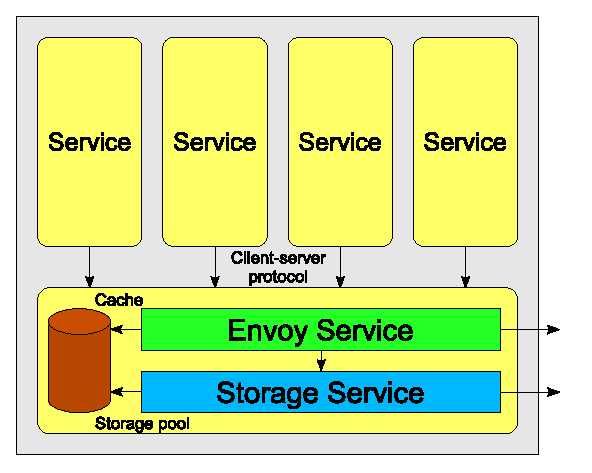
\includegraphics[width=\figwidth]{figures/single-machine}
\caption[Layout of Envoy services in a single machine]{Each physical machine has a single administrative VM that hosts the Envoy services. This VM exports a network file system protocol to other service VMs running on the same machine.}
\label{fig:single-machine}
\end{figure}

The file system management processes join a cluster-wide service that is comprised of two primary layers, as illustrated in \prettyref{fig:layers}. Storage is managed by the lower level, which allows a small set of basic file operations on objects. All operations are stateless and the storage service makes no attempt to prevent or manage concurrent requests or to enforce any kind of security policy. Objects are extents of bytes with a small set of attributes.

On top of the storage service is the envoy layer, which builds a hierarchical file system out of objects, coordinates access to files, provides authentication and access control services, manages caching, and exports a standard network file system interface for services to access.

\begin{figure}[tp]
\centering
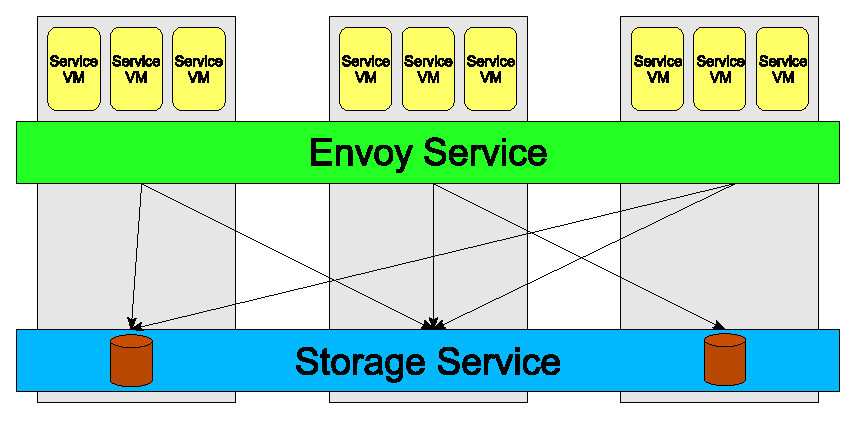
\includegraphics[width=\figwidth]{figures/layers}
\caption[The layers of the Envoy file system]{The envoy service coordinates access to provide a single, coherent view of the distributed file system. It relies on the storage service, which provides a repository of objects referenced by unique identifiers.}
\label{fig:layers}
\end{figure}

In the remainder of this section I detail the functionality and requirements of these systems and consider the tradeoffs of various design decisions.

\subsection{Distribution}

\prettyref{fig:client-server} depicts a commonly-used storage arrangement using a series of dedicated file servers to handle the needs of many clients. This architecture is successfully used in many settings and, despite alternatives developed over the years, is still the dominant storage model in practical use.

\begin{figure}[tp]
\centering
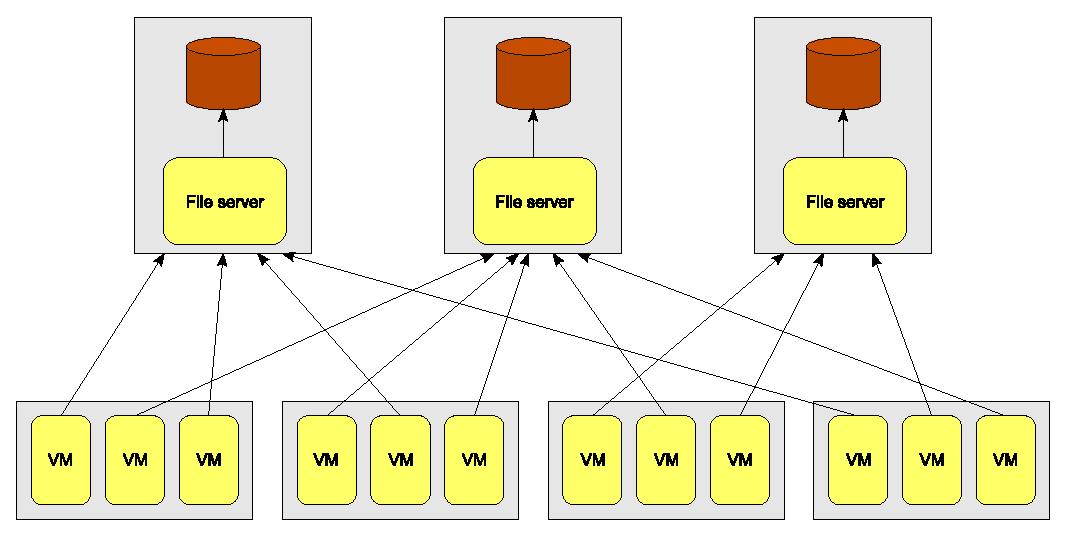
\includegraphics[width=\figwidth]{figures/client-server}
\caption[Machines served by a series of client-server file systems]{A popular storage solution for groups of clients involves a series of dedicated servers. Content on the servers is carefully managed to distribute storage demand and transaction load between the servers.}
\label{fig:client-server}
\end{figure}

The client-server model has obvious flaws when applied to clusters with many transient clients. Data placement decisions must balance space requirements and expected access rates in order to avoid overloading a particular server. Rebalancing---a disruptive and time consuming job---may be necessary in response to added clients, added servers, added disks, variations in client workload, and accumulation of data over time.

With the service cluster model, the problem is made even worse. To make efficient use of increasingly powerful hardware, each physical machine may host many services, each of which requires a boot image as well as access to the data relevant to its intended task. Dividing each machine means that there may be an order of magnitude more virtual machines than physical machines, putting excessive demands on a centralized storage infrastructure \cite{hospodor}. Single-purpose services may also be short lived or vary by time of data, making manual balancing impractical.

The client-server model has not endured as long as it has simply for lack of alternatives, however. It has many strengths that can inform the design of a more distributed architecture. With a single server managing shared data, concurrent access can be managed simply through explicit leases and cache invalidation, centralized caching with synchronous access, or through a lock manager. Whatever the mechanism for resolving conflicts, a centralized server is ideally suited to detecting and responding to concurrent requests because it is the point on the access graph at which all requests converge. The consistency of data that has reached the server is as good as its backing store.

The simplicity of a server is also a virtue. A failstop model for reliability can generally be assumed, backups are relatively straightforward, the server is typically dedicated to a single task or is shared with other trusted services, and the semantics are simple to define in terms of client behavior%
\footnote{NFS versions 2 and 3 have notoriously complicated consistency semantics, but this is almost entirely due to client policies. NFS server semantics are straightforward.}.

The chief faults of a centralized system are the introduction of a single point of failure and the inability to scale beyond the network and disk bandwidth that can be hosted by a single server. While these limits are unacceptable at large scales, they are quite serviceable for small groups of clients.

For clients that are sharing data, it is difficult to improve on a centralized server. For sufficiently overlapping data sets, any consistent model will degrade to something resembling a server during periods of contention because all interested clients will have to synchronize their access to the contended bits. A single arbitrator will ultimately oversee each bit of data, whether it is a traditional server, a lease-holding client, or a quorum of cooperating peers.

Sharing cache space is also a benefit of consolidated control of shared data. As the performance gap between disk access and memory access continues to grow, efficient use available cache space becomes increasingly important. Once again, a single centralized cache fails the scalability requirement, but a shared cache for a smaller set of clients with overlapping data needs provides attractive properties. Accessing a cache across a high-speed network is faster than accessing a local disk \cite{dahlin94b}, so in a cluster setting, organizing the aggregate cache around shared access patterns is more valuable than organizing it to localize access. Stated another way, the combined effective cache size of the entire cluster is greater when redundant entries are consolidated through sharing, and maximizing the combined cache size to avoid disk seek penalties is becoming more important than avoiding the network hops that arise from using a shared cache.

While a server cannot handle an unlimited number of clients, it can serve many clients under typical workloads. Scalability matters more at the level of the entire distributed system than when considering individual nodes. In the case of overlapping requests from different clients, a shared cache on a shared server will outperform a series of private servers, despite the overhead of network latency. Given that runtime contention is relatively rare \cite{kistler}, Envoy is designed to localize file ownership when there are no apparent conflicts, but to pick one participant to own files that are shared and act as a server to the others.

This principle of localizing control where possible, but reverting to a simple, well-understood client-server model when sharing is necessary is fundamental to Envoy. It leads to \emph{fate sharing} among clients with overlapping interests in the areas of performance, resource usage, and failure recovery. In each case, services with overlapping resource demands cooperate directly with each other and disinterested parties are not involved.

The overall distributed architecture of Envoy is modeled after human-administered systems using client-server file systems. Storage is distributed over a series of servers in an attempt to balance demand (the separate storage layer handles balancing capacity), but where a human administrator is constrained by practical concerns to using relatively few, well-provisioned servers, an automated system can continue the process of server division and balancing to a much more fine-grained level. Entire images or parts of images that are used exclusively by a single service (or a group of services hosted on a single physical machine) are managed directly by the envoy service on the same machine. Where sharing occurs, the client with the highest demand retains direct control and acts as a proxy for other clients accessing the same storage, thus sharing a cache and avoiding complicated coordination protocols.

\subsection{Storage layer}

\footnote{Citations to add: \cite{stein05}, HP trace shows that with caching, most operations that go to disk are writes, and non-sequential operations \cite{ruemmler}, so access patterns are probably less important in the layout of the storage layer than recovery concerns. chained declustering and correlated failure \cite{hsiao,lee96}. Object storage works well and is growing in popularity \cite{factor}. File layout doesn't matter as much behind the cache \cite{stein05}.}

The objective of the storage layer is to provide a simple, stateless interface for accessing objects. Redundancy to enhance availability and reliability and distribution to balance load is also handled by this part of the system. The storage layer is implemented in two parts, called the top and bottom halves.

The bottom half is implemented in the storage daemon hosted on each physical server. While the storage daemon instances form a collective pool of storage, they do not communicate directly with each other. At the local level, each storage manager is unaware of any global state, and responds blindly to incoming requests from the envoy layer. Instances do not attempt to balance load, resolve conflicting requests, or create redundancy, nor do they monitor which object IDs they considered valid. Instead, they provide a thin, simple storage service for numbered objects with attributes.

To make these servers more useful, the top half of the storage layer is implemented in the envoy daemon. It is responsible for mapping an object ID to the set of storage server instances that host the referent object. Combined with the persistent cache, the storage layer top half provides a simple procedural interface to the storage layer, where objects are named by unique IDs. The top half is responsible for creating and locating replicas, detecting and masking/recovering from failures, allocating new object IDs when needed, and reading and writing data and attributes.

An object ID is considered a globally unique name for that object. When replication is introduced, it is assumed that all replicas are given the same object ID. One object server from a replica group is nominated as the master; it is the only one to which \texttt{reserve} requests will be sent, and all servers within that replica group are bound by its allocations (although the servers themselves do not offer any enforcement mechanism). Object servers can participate in multiple replica groups, so the \texttt{reserve} procedure includes a parameter to indicate the ID space from which the allocation should come.

\subsubsection{Open problems}

The mapping of object IDs to specific storage servers is not defined in this work. Numerous strategies are available for distributing objects across the cluster, including random distribution, chained declustering, partitioning based on object ID ranges, co-locating objects created together, etc. For the purposes of this dissertation, I assert that an independent storage layer is viable and reasonable, but I do not discuss a specific system in detail. Other object storage systems of varying levels of sophistication could be substituted for the stub I describe here. The emphasis of this dissertation is on the envoy layer as implemented on top of the object layer.

\subsection{Envoy layer}

The envoy layer forms a file system from the objects provided by the storage layer, coordinating and caching access to the file hierarchy, and exporting a client-server protocol to services that act as clients of the file system. The entire cluster shares a global, hierarchical namespace, but clients typically mount a subtree from the hierarchy and treat it as a complete file system.

\subsubsection{Territories}

A single instance of the envoy service runs on each physical machine. The global name hierarchy is divided among participating instances in the cluster. When a given instance takes responsibility for some part of the namespace, it is said to \emph{own} a \emph{territory} covering the relevant subtree of the hierarchy. All operations within local territories are served locally and may be cached locally both in memory and in the persistent cache, which is reserved exclusively for territories local to the machine.

This partitioning of the global namespace and the resulting federation of constituent parts is what gives Envoy its name. When clients request operations that stray from the local territories, the requests are handed off to the envoy on the appropriate machine. It follows that each instance must know not only the boundaries of its own territories, but how to find the envoy for neighboring territories, i.e., those that can be reached by a single directory traversal (up or down) from a local territory.

The envoy service is stateful, and tracks not only its territories and neighbors, but the state of all files and directories in use by its client services. When a client navigates beyond the boundaries of a local territory, requests are forwarded directly to the owning envoy. If further navigation moves beyond the neighbor's territories, the neighbor does not forward it to the new envoy, but instead bounces the request back to the originator with the address of the envoy that can answer the request.

Under this system, two envoys maintain a direct relationship with each other only when they are immediate neighbors in territory ownership, or when one is serving requests for a client of the other. It follows that if territories are alloted such that the owner of a territory is also its most active user, traffic on an envoy instance will generally be dominated by its local clients.

Often, the best that can be achieved in a steady-state system is to have the owner of a territory be the envoy driving a plurality of traffic, not a majority. Sometimes this is an inevitable consequence of overlapping client demands, but often some further gerrymandering of the territory boundaries can restore a majority to the local territory. Since the needs of the clients and the needs of the envoys are generally aligned, a practice that in politics usually serves those in power at the expense of those they represent serves both equally well in file systems.

\subsubsection{Files}\label{sec:directory-format}

Files and directories can be mapped easily to objects as provided by the storage layer. Files are stored as objects with a set of attributes, and directories as files with special semantics and a different interface. Certain special files are stored as normal files with special contents, accessible through the interfaces appropriate to the file types.

Unix file systems are organized around \emph{inodes}, which encapsulate the contents of a file with its attributes, but not with its name. Envoy employs a similar structure, with file contents and attributes separate from the name hierarchy. Objects also have numeric identifiers like inodes, but it is worth noting that these identifiers can change during the lifetime of a file, so an object ID is not suitable for identifying a file.

Directories are files containing listings of other files. In Envoy, directories are managed at the block level, with each block containing some number of entries. An entry consists of a file name, the object ID that links to its contents and attributes, and a flag indicating the file's copy-on-write status. When this flag is set, the object is considered read-only, and will be cloned before any changes are committed to the file's contents or attributes. This process is completely opaque to clients.

Special files, such as device nodes and symbolic links, are stored as regular files whose contents follow a defined format. For symbolic links, the file contents are the target of the link, for devices they are an ASCII string identifying the major and minor device numbers, etc.

\subsection{Caching}

Citations: Most files in a file system (90\%) are never accessed after being created and as few as 1\% are used daily \cite{gibson98b}, so even a small persistent cache can be effective, and sharing the active files from boot images and the like will probably see heavy overlap: after all, moving only 1,000--10,1000 objects takes 42--77\% of the load with it \cite{klosterman} (reconcile this with \cite{muntz}). Another workload comparison \cite{roselli}. DBMS work also explores the idea of considering the aggregate cache capacity of the client-server system \cite{franklin}. Self-similarity in file systems \cite{gribble}. Speculative execution has been used to mask the latency of distributed file systems \cite{nightengale}, allowing improved performance without sacrificing cache consistency, and approach that compliments ours. Other work on consistency \cite{triantafillou,vilayannur}.

The cache design in a distributed file system must balance the needs for performance, consistency, and durability. While maintaining a coherent view of the file system that is tolerant to software and hardware faults, a cache should reduce latency, increase throughput, and increase overall capacity by reducing the network and disk congestion required by a given amount of activity and freeing input/output channels to absorb additional load.

Enhancing performance is the primary reason for employing a cache in the first place. The growing gap in performance between main memory and disk makes effective cache management critical, as a random disk access is five or six orders of magnitude slower than a similar memory access. Much work has been done exploring different cache replacement strategies, with significant gains to be had when future traffic can be predicted. Unfortunately, the service cluster environment does not provide any insight into the expected access patterns of its constituent services, as one of the purposes of the environment is to support arbitrary services.

In a 2002 interview \cite{spring}, the CEO of Google observed that for seek-intensive workloads, DRAM can be cheaper to deploy than disks. The seek time of a single disk cannot be improved significantly, so increasing overall disk performance generally requires adding redundant spindles. With many mirrored disks, many seeks can proceed in parallel and a random request can be satisfied fastest by the disk whose head position happens to be nearest the requested datum. Because the of the large performance gap, Google found it cheaper and faster to store their entire web search index in DRAM, which can serve many requests quickly, than to create enough replicated disks to handle the same transaction load.

While Google's implementation revolved around an inherently parallel task, it can still inform the design of a cache solution for Envoy. A single, commodity machine cannot hold as much memory as would be required for an index of the web, but by considering the aggregate capacity of a cluster instead of focusing on the capabilities of a single machine, they arrived at the surprising but sensible conclusion that ``it costs less money and it is more efficient to use DRAM as storage as opposed to hard disks''. Finding data in a local cache is ideal, but with a high-speed network connecting machines in a cluster, it is faster to query the cache of another machine than a locally-attached disk \cite{dahlin94b}, suggesting that it would also be prudent for the design of Envoy to consider the combined cache of the cluster as well as the cache of individual nodes.

Envoy is designed to compromise between the competing goals of maximizing local cache hit rates and maximizing the aggregate cache capacity of the cluster. Two design features are particularly relevant to addressing these goals. The first is that all client requests are served synchronously by the envoy service without the aid of a local cache. Instead they rely entirely on the shared cache hosted by the envoy service in its private virtual machine. The local envoy directly services all requests---local and remote---for territories it owns, so the entire cluster caches at most a single copy of a given file.

This could potentially strain the envoy that owns a particularly popular file, as it funnels all traffic for that file to a single node. For light to moderate sharing, this is not an issue, and in practice the envoy will be accessing the file mainly from its cache and can handle significant traffic. For extreme instances of sharing, I argue that services should use explicit network-facing protocols instead of relying on the file system as a \emph{de facto} distributed shared memory system.

The second design feature has a more complex impact on the aggregate cache capacity. Territorial boundaries are drawn along boundaries in the namespace hierarchy, but because of the copy-on-write mechanism in snapshots and file system forking, multiple names may refer to the same underlying storage layer object. This only happens when the object (but not necessary the file) is read-only, so cache consistency needn't be considered, but it does mean that multiple envoys may cache the same underlying object. While this mechanism introduces redundancy in the cluster-wide cache, it also has the potential to consolidate cache entries within a single envoy instance. If multiple services are using different files backed by the same object, they will occupy the same place in the persistent cache as well as the in-memory cache.

Cache utilization is most effective when clients on a single machine use file system images forked from a common root, and the more complete the root image the more likely it is that services will rely on common rather than custom-installed files. This fits nicely with the stated goals of flexible commodity computation, where both the host and the client gain from using the most popular commodity tools. The host by reducing client footprint and increasing capacity, and the client by reducing deployment costs and maximizing performance through increased cache hits.

\subsection{Data paths for typical requests}

To summarize the architecture of Envoy, consider the data paths followed by typical file system requests as depicted in \prettyref{fig:hops}. The best case (retrieval from in-memory cache on the same machine) is designed to be the most common, with extra steps being required in progressively less-common operations until the worst case, where a request travels from a client to the local envoy service, is forwarded to a remote envoy, misses the local cache and is forwarded to a storage server instance where the data is retrieved from disk.

\begin{figure}[tp]
\centering
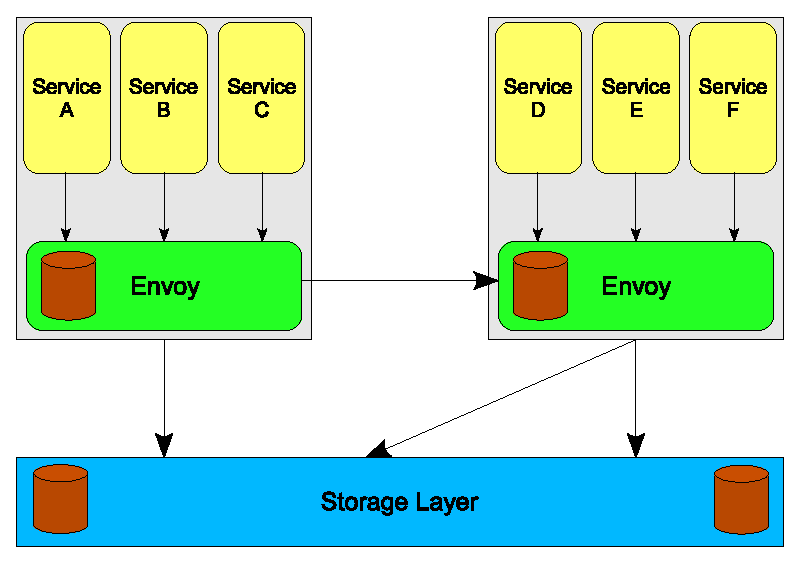
\includegraphics[width=\figwidth]{figures/hops}
\caption[Network paths taken by typical file requests]{File system requests proceed from service VMs to the local envoy service. A request from a local territory may be filled by the local in-memory cache, the local disk cache, or by a single network hop to a storage server. A request for a foreign territory adds a single network hop in each case, as the local envoy acts as the client to a remote envoy.}
\label{fig:hops}
\end{figure}

\subsubsection{Read operations}\label{sec:data-paths-read}

The best case is a request for hot data in a local territory. In this case, data can be served from the in-memory cache of the local envoy server. With a fully optimized implementation using Xen or a similar VM environment, this data transfer can occur with a single data copy from the cache to a data page, and that page can then be swapped directly to the client VM via page table manipulation. Since the client's OS does not keep a cached copy, that page can likewise be passed on directly to the client application. While my prototype is not this optimized, the design permits a very lightweight operation involving a single data copy and some metadata manipulation.

Warm data from a local territory follows a similar path, prefaced by retrieving the requested data from the local persistent cache (on disk) into the in-memory cache. With large, cheap commodity disks, the persistent cache can easily hold several operating system images and typical application suites. Typical Linux installations occupy no more than a few gigabytes, and even that includes many supporting files that are rarely used and may never be referenced in common service deployments. If services have forked from standard base images as proposed, it is realistic to assume that the entire operating system and standard applications will be available in the local cache hierarchy for a service being deployed on an active node.

When the local cache fails to deliver, the envoy service must retrieve requested data from the storage layer. The top half of the storage layer provides a complete object server catalog, so a request can proceed in a single network hop to the node in the storage layer bottom half that hosts the needed object. For simplicity, the persistent cache holds only complete objects, so an entire object must be transfered before the envoy service can begin fulfilling requests from the local cache. If the object is replicated, the envoy stripes the transfer across the servers, e.g., if there are three replicas, it streams the first third of the file from the first server, the middle from the second server, and so forth.

Operations in territories outside local control add an extra network hop between the local and remote envoys for all operations. The data also bypasses the local cache, so locality of reference does nothing to remove this network penalty. It does offer another optimization opportunity (the data, once received from the network, can be passed to the client application without any further copying) but this is minor compensation for a guaranteed latency penalty.

Fortunately, this penalty need not be too great nor too common. The remote envoy handles the request just as it would one from client local to it, including caching, so referential locality does improve performance from the cold-cache worst case. The target environment is service clusters, too, with high-speed local area networking and unmetered inter-node traffic. Finally, because of the way territories are decided, in a steady state system foreign envoy requests generally imply some degree of sharing. While relatively uncommon in itself, genuine sharing requires \emph{some} form of synchronous network communication to guarantee consistency, so Envoy's goal of reducing synchronous inter-node to cases of either sharing or infrequent access seems a reasonable one.

\subsubsection{Write operations}\label{sec:data-paths-write}

Citation: Transactions, strengths and weaknesses \cite{gray81}.

Write operations are less common than reads, but much of the complexity in file system design comes from supporting them. While a good cache satisfies many read requests from memory quickly and with no correctness concerns (provided coherency is maintained in the case of distributed systems), write operations cached in memory raise concerns about durability. If the server acknowledges the write operation as being complete but has only committed it to an in-memory cache, then there is a window of vulnerability before the data is stored to disk and all metadata updated wherein a system crash could lose data that the client expects to be resilient to crashes. In an isolated client, this may be acceptable as the client will simply be forced to restart from the state that was committed to disk and will generally only lose a bounded amount of work. It is particularly problematic for distributed systems and others with external side-effects, however, where other participants may cue subsequent actions on the premise that a write has been successfully and durably committed to disk. The problem is further exacerbated in a commodity hardware environment where failures are routine.

At the other extreme, one can commit all writes to disk before completing the transaction. This makes it clear to the client when a write operation has been consummated, and it is free to either wait for the acknowledgement or proceed asynchronously with explicit knowledge of the risk it is assuming. While this is a simple and appealing model, it ignores two important realities. The first is that the default action for most commodity operating systems is to cache writes and acknowledge them immediately while delaying the disk write. Changing the expected performance characteristics of a basic operation like writing to disk would not provide a commodity-friendly environment as it would severely affect the performance of many standard tools in a negative way. The second is that most files created are short-lived temporary files that are soon deleted \cite{ousterhout}, so synchronously writing them to disk introduces not only unnecessary latency but also unnecessary disk contention.

Several intermediate possibilities exist. Instead of having write requests proceed directly to the storage layer, the local persistent cache could be used as a staging area, with write requests being committed locally and then forwarded to the storage layer after some delay. This would do little to improve performance, however, as synchronous disk access is slower than synchronous network access, so this would not eliminate the slowest link in the event chain. Specialized hardware with involatile memory could also act as a staging area, giving good write performance while retaining durability. The latter approach violates our goal of using widely-available commodity hardware, however, and neither approach is resilient to hardware faults that result in the entire node failing.

Another approach is to only guarantee synchronous durability when explicitly requested by the client, using the equivalent of the Unix \texttt{fsync()} system call. This matches the semantics of local file systems, and thus what most software is written to assume. It is not without faults, however, as the popularity of high-level scripting languages and middleware frameworks (especially for network services, exactly the types of clients service clusters are designed to support) means the connection between application actions and disk operations is often obscured. Requiring low-level controls to get correct behavior is often an acceptable compromise, but it is rarely ideal.

The solution Envoy employs is based on exploiting the cluster environment. While commodity hardware is expected to fail occasionally, simultaneous failure of multiple machines is still relatively rare, provided that the nodes are sufficiently isolated from each other in terms of power and cooling. Since service clusters are intended for professional hosting environments, it is reasonable to assume that hardware faults occur in isolation. With that assumption, durability is less about committing data to disk and more about redundancy. A write request is considered final when it is in the memory of all of the storage servers that will eventually commit it to disk. If the envoy server fails, the storage servers are unaffected. If one or more of the storage servers fails before committing the data to disk, the recovery mechanism must restore consistency using the most up-to-date of the replicas. Having storage servers potentially out of sync due to a failed asynchronous write in this scenario is fundamentally no different from having one fail while trying to satisfy a synchronous request. In both cases, the inherent asynchrony of the network means that only the degree of the problem changes.

\section{File system images}

A single, hierarchical namespace unites all the participants in an Envoy cluster, but for management purposes there are two distinct levels. The administrative file tree starts at the root of the namespace and has as its leaves the file system \emph{images} that are normally accessed by clients. Imposing this additional structure in the tree codifies the intended usage pattern, which simplifies administration and allows for some simple but effective optimizations.

\subsection{Security}

Service clusters must accommodate a heterogeneous collection of clients, some of which may trust each other, but most of which will not. To support standard operating systems and tools, Envoy must support familiar semantics, including granting complete control over private images, while also accommodating shared images that grant limited access to various clients. In addition, clients themselves may wish to arbitrate access to shared storage, rather than expecting the cluster owner to provide a sufficiently rich sharing model for any combination of services.

\subsubsection{Enforcement}

Simple security is one of the benefits of the service cluster model. Physical machines are controlled by trusted software that isolates clients from each other and from the administrative tools. Having the cluster in a managed environment similarly secures physical access to the machines and makes a trusted environment possible. Virtual network devices connect client VMs within a machine, and they also route network packets from clients to the rest of the cluster and the outside world. With well-defined and controlled boundaries, packets cannot be spoofed and network addresses can be an accurate and reliable indication of the origin of network data.

For Envoy, this means that client access to the file system can be strictly isolated to the client-server interface exported by a client's local envoy. The clear lines of trust provided by the environment make enforcement of security policies relatively simple. Envoys communicating with each other can be authenticated by their network address as well as by the credentials they provide, as can connections between envoys and storage servers. Encryption of traffic is possible, but since the cluster contains only trusted machines, the threat of packet sniffing is much less than in other environments.

\subsubsection{Policy}

When a client mounts a directory, be it a file system image or an administrative directory, it supplies its credentials and the pathname of its root directory relative to the global root of the file hierarchy. Envoy evaluates the supplied credentials relative to the directory that the client is attempting to mount. If permission is granted, then the client can access that directory and any of its descendents with the level of access it was granted at mount time.

The credentials required to access a given directory are determined by the contents of files called \texttt{password} located in the administrative directories above the target directory. The access granted by each level is additive, i.e., permissions can only be added by a new \texttt{password} file, not taken away, and normally applies to all subdirectories that are siblings of the \texttt{password} file, not to the directory that contains it. The root of the entire tree is an exception, as its \texttt{password} file applies to the root directory as well as its descendents. The significance given to \texttt{password} files only applies to administrative directories. Once the boundary to an image has been crossed, all special names recognized in the administrative directories cease to have significance.

The lowest level of access granted by a \texttt{password} file is read-only or read/write access to images. This allows clients to mount images and use them, but grants no access to the administrative directories. The next level up lets the client mount administrative directories to trigger and manage snapshots, but not create new images or manipulate other files in the administrative areas. The highest level of access permits these activities as well, giving clients the ability to manipulate lower-level \texttt{password} file as well. To fork an existing image, the user must also have read permission to the complete base image.

Credentials can be restricted to grant access as a specific user name in the file system, or they can be mapped to any user within an image. The latter case is analogous to the \texttt{root} user in a Unix system, which can assume the identity of any other user within the same system.

With this system, a few typical user types are expected:

\begin{description}
\item[Service managers] coordinate groups of client VMs that cooperate to form larger services. They create new boot images, set up shared volumes, and grant appropriate access to the individual participants.

\item[Client owners] act like root users for a particular image. The client may create its own user names, but instead of registering them individually with the file system, the client owner uses its own credentials to authenticate them and grant them a name for the duration of the active session. Client owners may also manage their own snapshots.

\item[Independent users] may be authorized by service managers to access individual shared volumes within their management domain, without granting them \emph{carte blanche} or putting them under the control of individual client owners. These free agents are guests in the images they visit, but their access may come high in the file tree giving them access to many images.
\end{description}

Other roles may be created with the system. The objective is to make it simple for individual users, allow clients to manage their own user base in shared setups, and allow restricted access to be granted by clients to other clients for sharing.

\subsection{Forks and snapshots}\label{sec:snapshots}

To support the rapid deployment of services, standard installations of commodity operating systems and software can be provided to clients as a starting point. This is accomplished in Envoy by creating a small set of well-known base images and allowing clients to fork them as a starting point for their own private images. Using copy-on-write techniques, many clients can diverge from a single image, sharing unchanged files and consuming resources only for the changes made.

The copy-on-write mechanism in Envoy works at the level of an object in the storage system. Files and empty directories are leaves in the object tree, with non-empty directories acting as interior nodes that branch out. Modifications to privately-owned objects can be made directly to those objects, but changes to a shared object can only be made by cloning it and applying the changes to the copy.

An object clone has a different object ID than the original, so directory links to the object must be updated, which in turn may require cloning the directory object. Changing a leaf in the file system tree requires cloning a path from a writable ancestor to the object itself, a process that resembles modifying an immutable tree structure in a functional language: an entirely new tree is produced that links back into the old tree whenever possible.

\subsubsection{Image versions}

While snapshots could be taken at any point in the file hierarchy, a few additional rules simplify management. The root of the namespace is always writable, as are all administrative directories, i.e., those that are not descendents of a directory called \texttt{current} or one of its numbered snapshots. Existing snapshots are always immutable, and new ones can only be taken from the root of an image, not from arbitrary points in the client's directory structure.

A new image is started by creating a directory called \texttt{current} in an administrative directory that does not already contain an image. The active version of the image retains that name, while snapshots are named as successive positive integers. This process restricts the history of an image to a linear progression of snapshots taken over time. For management purposes, the entire collection is considered a single image with an active head rooted in the \texttt{current} directory and a series of historical versions.

\subsubsection{Forking an image}

The word ``snapshot'' implies that a copy of the state of an image is frozen and set aside as an external observation of the active system, but in reality it is the active version that is frozen and set aside, while a newly-created head takes the place of the old one and diverges from it over time. The continuity of the active image is preserved through sleight-of-hand as active file state is transparently transferred from the old head to the new.

The process of forking an image is the same, except that it starts with a snapshot already frozen as part of the history of another image. To fork a running image, a snapshot must first be taken, after which the forked image and the new head of the old image can both start from the same immutable tree and move forward independently.

\subsubsection{Snapshots and territories}

Because of the copy-on-write mechanism, changing a single file may require modifying a path all the way back to the root of the image, potentially crossing territory boundaries and involving multiple envoys in the process. This would violate the goal of local impact for normal file operations and complicate the protocol between envoys. To simplify matters, Envoy requires that the root of each territory be writable unless it is part of a read-only snapshot. The worst case is reduced from cloning a path back to the root of the image to cloning a path to the root of the territory, making it possible for write operations to be completed by a single envoy.

To satisfy this requirement, the snapshot operation must clone a path to each territory exit after freezing the territory. In practice, snapshots operate on the territory tree from the leaves to the root. Child territories are frozen and their roots cloned, then parent territories are frozen and paths from their roots to their children cloned. Eventually, the root object of the image is replaced by a clone; the old object becomes the root of the snapshot and the new clone becomes the root of the active head of the image.

This process simplifies writes, but it also creates unnecessary cloning for territories that do not serve any write requests before the next snapshot. This is a tradeoff between simplicity of design and space efficiency. Cheap and ample disk space is one of the motivating advantages to using commodity hardware, so this tradeoff is consistent with the goals of the Envoy file system.

\subsection{Deleting snapshots}

Storage space is cheap and plentiful, and systems such as Venti are designed to keep a complete history of all files ever created \cite{quinlan}. This may be appropriate for some workstation environments, where the increase in storage capacity can out-pace typical data creation rates, but deleting files permanently is still a necessity for many other users. In service clusters, users are charged according to the resources they use, so they must have the flexibility to completely remove old files. Also, when clients leave a particular service cluster, the owner may wish to reclaim the space for future use, as there is little incentive to keeping it around on behalf of a client that is no longer paying. Also, concern for privacy and compliance with data retention laws may require data to be completely removed.

Backups in Envoy are done through snapshot operations, and anything created and deleted in the window between two successive snapshots is no longer accessible anywhere so it is deleted immediately (with an exception described in \prettyref{sec:hard-links}). This is easily detected through the copy-on-write mechanism, which identifies all files that were created since the most recent snapshot. All files with copy-on-write flags (either explicit in a directory link or implicit through an ancestor's link) are backed by objects referenced by one or more read-only snapshots, so envoys never delete these objects when their corresponding files are deleted.

The problem comes when trying to delete old snapshots, as it can be difficult to determine which storage objects are used only by the files in a given snapshot.

One obvious solution would be to implement reference counting in the storage layer. This has the advantages of simplicity, accuracy, and immediacy. The main disadvantage is that it puts the performance burden in the wrong place: every time a directory object is cloned (an frequent operation after a snapshot as the copy-on-write mechanism supports write requests) the reference count for all objects in that directory would need to be incremented. This would require clone operations to be implemented in the envoy layer which can locate all object replicas, or the bottom half of the storage layer (where clones are implemented) would need to be aware of the topology of the entire storage layer, a requirement currently confined to the top half. In either case, a lot of extra traffic would be generated to support an operation that is relatively infrequent and not timing critical.

The copy-on-write mechanism in Envoy is similar to the one I implemented while working on Parallax \cite{warfield}, as is the problem of deleting snapshots. The problem was simpler in Parallax, however, which uses a copy-on-write radix tree to map logical blocks to physical blocks in a virtual block device. The virtual block numbers do not change between snapshots, so comparing the physical blocks mapped to by two successive snapshots reveals which blocks from the first were unlinked during the lifetime of the second.

With Envoy and its hierarchical file tree, the problem becomes more complex. Comparing two successive snapshots is no longer straightforward, because files and directories can be renamed. The virtual block IDs that are static in Parallax are replaced by variable names in Envoy, making the process of comparing two snapshots more difficult. Supporting hard links makes it even more difficult to define a one-to-one correspondence between object references in two successive snapshots.

This potentially messy problem can easily be solved by brute force. Instead of imposing extra runtime overhead for normal file operations or attempting to walk two file systems and identify matching files within them, it is simple and practical to gather a complete list of objects referenced by an image. Using 64-bit object IDs, such a list would take 8 megabytes for every million files. In a 1999 study of workstations at Microsoft, Douceur and Bolosky found an average of 13,309 files over 10,568 machines, with the subset running NTFS (the newest file system studied and the one with the largest average number of files) averaging 24,229 files over 3332 machines \cite{douceur99}. This number will no doubt continue to grow, but anecdotal tests found the number still in the low millions for typical, modern Linux desktop installations.

Just as high-level languages are worth using despite being slower and using more memory than lower-level languages, I consider the simplicity of gathering a complete list of objects and sorting it to outweigh any potential performance loss compared to a more sophisticated but more complex approach. For problems like this one, it is not even the relative performance or storage requirement that is salient, but the absolute size: deleting snapshots is not a critical path operation and for typical image sizes the brute force approach is cheap enough that no amount of optimization would be worth more than a very small complexity increase (Amdahl's law \cite{amdahl} is relevant here, but the ability to execute the operation asynchronously makes any (reasonable) cost even less important).

A sorted file with all object IDs referenced in the snapshot can easily be stored in the administrative directory that contains the image. To delete a snapshot, the objects of it and its immediate successor and predecessor are compared in order. Each object that appears in the snapshot but disappears in the successor can be safely deleted from the storage layer. To make it safe and resilient to crashes, the envoy service ensures that no clients are currently accessing the snapshot, then it unlinks the root of the image first, and deletes the list of object IDs last. At recovery time, an object ID file found without a corresponding image indicates that a crash occurred before the operation completed, and it can be safely restarted. The image itself isn't necessary at this stage, and as long as the cleanup process can tolerate objects having already been deleted, it can work entirely from the object lists.

The only other complication in this process is image forks, where multiple successors may exist for a single snapshot. Forking an image does not directly affect the snapshot used as the starting point, so the easiest way to detect forks it to log them. The log is consulted before any snapshot delete attempt, and deleting images that have more than one immediate successor is not permitted.

A few other corner cases are worth mentioning. The current version of an image can be deleted using the same procedure, but it must be made read-only or client access must be disallowed before gathering the list of object IDs (note that access is normally only forbidden when deleting starts, as the catalogs of predecessors and successors must be assembled as well as those of images marked for deleting). Otherwise, the normal procedure suffices, with the successor object catalog taken to be empty. The log of image forks also needs to account for deletes, so that entire trees of images can eventually be pruned back to the root if desired.

\section{Territory management}

The Envoy file system model is based on the idea of presenting a single, large file tree connecting arbitrary images, but providing incentives to use it in ways that can be exploited to provide good performance and scalability. The service cluster model makes it simple to isolate control of the file system from the clients who use it, while still keeping synchronization logic and caching on the same machine most of the time. Providing a global namespace gives a great deal of flexibility, but inferring usage patterns and co-locating ownership of branches of the tree with the clients that use them yields short data paths and good performance.

\subsection{Design principles}

A variety of approaches to distributing territory ownership are possible, and only a realistic usage model drawn from empirical study of real-world deployments can accurately inform optimum choices. Lacking that, territory management in Envoy is designed around a few principles:

\begin{itemize}
\item Optimizing long-term patterns is more important than following short-term trends. High-speed switched networks minimize the penalty for serving a request from a remote envoy compared to handling it on the client's envoy, and the growing gap between memory and disk performance makes flushing the cache with a territory move continually more expensive. Based on this and on the past success of client-server file systems, Envoy favors slow evolution of the namespace topology to capture steady-state client behavior. Instead of attempting to track each change in runtime usage patterns, it offers a client-server model that gradually optimizes itself over time by co-locating servers with clients.

\item Simplicity is a virtue. This applies to the runtime behavior of the system as well as the algorithms and implementations that drive it. For debugging, recovery, and runtime analysis, territories with simple boundaries that do not change frequently are preferred. Painting the namespace tree in broad strokes makes it easier for humans to comprehend and analyze, minimizes perverse cases that can threaten correctness and the success of recovery operations, and makes global logging of changes practical. With this in mind, Envoy favors using a few territory divisions to give good results over making many divisions in an attempt to approach optimal results.
\end{itemize}

\subsection{Special cases}

Many systems use leases to coordinate access to file system objects as a form of token passing. When a client wants to access a file, it must first gain control of the file, and it must transfer control to a second client before it can operate on the same file. This may be limited to write operations, allowing a window of delay before updates are visible to other clients, but in either case the transfer of control happens in real time before a request can be satisfied. While these operations can be optimized, fundamentally they operate on a pessimistic model similar to mutex locks in shared memory schemes.

Territories in Envoy are analogous to leases and token systems in many ways, but they are based on an optimistic model where large groups of files can be granted to an owner on the assumption that sharing is uncommon. Every request from a client can be processed immediately either by the client's envoy or by a direct, already-established link to the owner, with complete access to the owner's cache. In this way it is more like a set of manually configured servers that are dispersed throughout the cluster than a set of lease-holding clients with equal claim on an object. Performance is best when the server is on the same machine as the client, but it is not bad when an extra link is introduced.

The decision to cede all or part of a territory to another envoy is always made by the current owner. While a client's envoy may be able to recognize the client's ongoing demand for a particular region of the file tree, only the envoy that manages it can account for all clients that are accessing it and act based on complete information. Transfers are always driven by the parent of the root of the branch being transferred, but the parent only initiates a transfer when the owner of the branch requests it. This leads to the first special case in territory realignment: when a territory is dormant, it is ceded to its parent. Dormancy is determined through the general mechanism described below, but this is highlighted as a special case because no other envoy can detect a territory that has fallen out of use. Territories are also ceded when an envoy is shutting down.

Another special case is based on the expectation that most images (especially those used as boot images) will be used by only a single client: when a client mounts an image that is not in active use, the image is immediately ceded to that client's envoy. The first client to mount an image may not be the one that expects to use it the most, but it is more likely to do so than the owner of the parent, which may have no interest at all in the image. For services with no sharing, this heuristic by itself is sufficient to completely localize non-administrative traffic. This is also an example of how imposing a little structure on the file tree can not only simplify administration, but also improve performance.

\subsection{Dynamic boundary changes}

Control of a private image is handed over the the relevant envoy when the client mounts it, but control of shared images is initially given to the \emph{first} client to access it, which may not necessarily be the heaviest user. Envoys observe the access patterns of their local clients and compare them to forwarded traffic from remote envoys, periodically ceding control of parts of territories, or even handing over control of an entire territory in an attempt to improve locality of access.

Territories are transferred in response to observed usage, with one of two goals: to improve locality or to simplify the territory layout. The latter occurs when traffic to a territory falls below the \emph{idle threshold}---a configured value---and the benefits of local ownership are not considered worth the extra cost in topological complexity. In this case, the territory is handed to the neighboring envoy with the most boundaries in common with the old owner, either the parent or the owner of one or more children territories.

Traffic is monitored by the number of requests from each remote envoy, with all client requests combining to form the owner's contribution. A single value for each participant is computed as the total number of requests, exponentially decayed over time with a configurable half-life. This approach allows envoys to continually monitor load and react not only to the presence of imbalances, but to their severity as well. Sub-optimal layouts are addressed more urgently when traffic volumes---and the potential benefits of optimization---are high, and a slower response in low traffic, where waiting can confirm that the trend is lasting and that a fix is likely to be worthwhile.

For simplicity, only a single new territory is created in each realignment; if two branches of a territory need to be ceded to a remote envoy, they will not be combined into a compound transfer, but will instead be evaluated and transferred independently. To aid in accurately predicting the effect of a given transfer, the traffic value for a directory combines requests for its descendents with those for the directory itself. With the assumption that recent trends will continue, the combined traffic value for a particular object will summarize the overall effect of ceding it as the root of a new territory.

For each object in a territory, the owner considers ceding the branch rooted at that object to each envoy that has driven traffic to the branch. The harm to the local envoy and the benefit to the remote envoy are weighted equally by subtracting local traffic from that envoy's traffic to compute the expected benefit of a transfer. Requests from third-party envoys will be unaffected, as they will just be transferred from one remote envoy to another. In this way, the expected benefit of each territory change (including transferring control of the entire territory) can be considered and compared with the alternatives.

Before actually initiating a transfer, two conditions must be met: the transfer must be the one that will yield the maximum expected benefit, and the elapsed time since the most recent change to the territory must be inversely proportional to the expected benefit of the new change. A highly beneficial transfer is considered urgent, but if the improvement is modest then it is delayed to encourage stability in the topology and discourage thrashing of the cache.

Scanning an entire territory after each request would be prohibitively expensive, but the scheme outlined here can be approximated in a straightforward fashion. As each request is recorded and the traffic value for affected objects updated, the envoy computes the expected benefit of transferring that object to the originator of the request. This process is repeated as the request is recorded for parent directories all the way to the root of the territory. The maximum benefit observed is compared to the time elapsed since the most recent transfer, and the envoy can then decide if a new transfer is warranted.

A transfer that was rejected at the time of a request for insufficient magnitude may become viable as the territory ages, and the envoy will not notice it in the absence of a new request to trigger a re-evaluation. While this would violate a strict interpretation of the procedure, it would do so only in the absence of traffic from the remote envoy, a condition that would cast doubt on the efficacy of the transfer anyway.

\section{Recovery}\label{sec:envoy-recovery}

Putting commodity computation in a managed environment with well-provisioned hardware reduces the rate of node failure, but all computer systems are subject to the risk of failure, whether from hardware faults or software problems. A viable recovery procedure is essential for any storage system, and minimizing the disruption to other nodes is also important in a cluster environment.

The controlled environment has its advantages, however, in that the expectation of failure for a given node is low enough that it can be treated as an exceptional condition, rather than a normal part of operation. This stands in contrast to distributed systems running on machines owned and managed by a wide range of people, whether peer-to-peer systems on volunteered machines or networks of workstations in a corporate environment, where the needs and habits of the owners preempt the interests of the whole system.

As a commodity platform, failure of an individual node can reasonably disrupt the services running on it. Uptime guarantees and other reliability requirements must come from higher-level services, which may be implemented as a series of clients on a service cluster or across multiple clusters. The latter is necessary for the most stringent requirements anyway, since catastrophic failures such as natural disasters may affect all machines at a location no matter how well cared for. Since prevention of failure is impossible, and failover capabilities for all clients would be complex and expensive, a more practical approach is to assume that nodes will occasionally fail, and seek to minimize the disruption to the rest of the cluster while restoring the service of the lost node as quickly as possible.

The basic assumption implicit in Envoy's recovery model is that the failure of a machine or any of its parts (including management software) may result in lost service to the clients hosted on that machine. Moving outward, envoys that were interacting with the failed machine should be able to recover fully with some disruption, while nodes that had not overlapping interests should be unaffected.

The other philosophy that drives failure recovery is that it should be as simple as possible. Recovery scenarios are both difficult to predict and difficult to simulate. In a distributed system, interactions involving multiple participants can be complex enough when they work, and an unanticipated failure at an unexpected time can often lead to conditions that are hard to anticipate. Enumerating cases that must be handled is an error-prone process that can become intractable with too many sources of faults. Even when complex failure cases are correctly identified, simulating under realistic conditions to test equally complex recovery code is another difficult and error-prone process. Ongoing field testing is dominated by correct behavior (one hopes) so recovery code is rarely exercised as well as normal code paths. Finally, because recovery procedures are only invoked in response to failure, they represent the last line of defense against lost data and the last chance to retain the trust of users, a critical element in storage systems.

Some of the most successful systems reflect these concerns. Database systems typically log transactions in a simple, append-only structure before applying changes to complex data structures. At recovery time, no attempt to diagnose the exact conditions of failure is necessary---instead the log can be replayed to complete committed transactions or even an interrupted recovery process. Similar journaling schemes are increasingly common in modern file systems for many of the same reasons. Careful ordering of writes can ensure that a crash at any stage leaves the system in a sane state, offering the same principle benefit: recovery from a wide range of failure conditions can proceed even without knowing what actually caused the failure.

\subsection{Prerequisites}

Some amount of redundancy of runtime state is necessary to allow complete recovery after a node failure. The fate of a client is already tied to that of its local envoy, so envoys track the state of all active file handles for local clients, including those files that are owned by remote envoys. The local envoy acts as a proxy server for remote files, so it can easily peek at request and reply messages to observe state updates. For local and remote file handles, an envoy tracks the full pathname of the file, the user credentials used to access the file, and any state related to file status and position required to support the client-server protocol exported to the client.

A client's envoy can track its file handle state locally, but file data is not duplicated for forwarded requests. Duplicating runtime state can prevent disruption, but preventing data loss requires redundancy in written data and attributes. The write-through persistent cache in Envoy answers this requirement by ensuring that data has reached the storage servers for all replicas before reporting a write operation as complete. As long as the relevant storage servers are able to carry on long enough to write the data to stable storage, the crash of an envoy node will not affect the stability of data, nor its immediate availability to the recovery process.

Depending on the storage layer implementation, a window of vulnerability may exist between the time the first and last storage servers have been notified of an update, during which an envoy crash would result in an inconsistent state between replicas. The problem resembles that of a storage node failure, and in both cases recovery of the storage node would necessitate it ``catching up'' with missed transactions. This is fundamentally a part of the storage layer design, and as a detailed discussion of object storage strategies is beyond the scope of this dissertation, I omit further discussion of solutions to this problem.

\subsection{Process}

With runtime state and file data available, it is possible for envoys that were interacting with a failed node to recover fully from the disruption, with temporarily degraded performance as the only effect visible to clients. The affected envoys include all those with which the crashed node had any kind of relationship, including the owners of the parents of its territories, the owners of the children of its territories, remote envoys accessing files in its territories, and remote envoys to which it is forwarding requests for local clients.

The first step in recovery is recognizing that something has gone wrong. Envoys monitor the status of their neighbors in the territory tree as well as that of the envoys with which they share files. These connections can be monitored closely without imposing a significant burden on the network, as they are always unicast messages between small sets of hosts. Normal interactions can double as heartbeat messages most of the time, and explicit messages are only necessary on otherwise idle connections.

Once a node fails, the territories it owned and their descendents are immediately dissolved and annexed into the parent territory. In-flight operations no longer act under the authority of a territory owner and are suspended. Forwarded operations between two otherwise-healthy envoys are rejected with a suitable error so that the client's envoy is made aware of the failure. Parents notify children recursively, resulting in a pool of envoys that hold file handles for their clients but have nowhere to send transactions. The envoys then reconnect each file handle to a territory owner by walking from the root of the file system tree to find the new owner. Unlike normal directory navigation requests, these traversals always succeed, even if directory permissions have recently changed. Envoys can also nominate themselves to reclaim ownership of territories, or they can leave it to the normal demand-driven process to sort out boundaries over time.

In keeping with the goal of simplicity and blanket coverage of failure cases, this handles failures that occur in the middle of territory ownerships transfers as well as simpler, steady-state cases. The canonical version of the file tree is maintained by the storage system, not by the soft state of territory ownership. Once the ownership tree is corrupted by a failure, the corrupt branch is pruned and re-grown from its former root. Similarly, the canonical version of a file handle is maintained by the client's envoy, not by the territory owner. Envoys champion the needs of their own clients by restoring their file handles to working status and resuming their suspended operations, while the operations initiated by failed envoys are forgotten and their files implicitly closed.

If a snapshot was in progress when the failure occurred, it is possible that orphaned objects may result. The snapshot can still succeed, because the change at the root automatically covers the entire branch, but objects that were being cloned through the copy-on-write mechanism, either to permit a file write or to maintain writable territory roots, may be lost due to a failure. Directories and their links to objects are updated after objects are successfully cloned, so this will not result in a data loss, but it may leave an occasional object that cannot be reached through the file tree. The potential for minor capacity loss is regrettable, but should not be the source of too many tears.

\subsection{Special cases}

Throwing away damaged soft state and rebuilding it instead of trying to patch it makes recovery from a node failure simple and uniform across a range of failure conditions. An important step in the process depends on the ability of newly-ostracized envoys to rejoin the collective by starting at the root of the tree and pushing file handles back down to their appropriate locations. Two problems can inhibit this process: failure of the root node, or a change in the path from the root to the target node.

Every node that joins the Envoy system must know how to locate the root node. Whenever a client attempts to mount a file system image, it specifies it as the path from the root of the global namespace to the root of the image. Locating the root initially may be part of the startup process for an envoy, or it may integrate more closely with a higher-level service-cluster management tool. Other management services must exist to instantiate and monitor client VMs, and it is sensible to have Envoy coordinate directly with those services. Monitoring the root node and anointing a replacement when it fails could fall to the management tools as well, or envoys could instead be started with an ordered list of root nodes, the next taking over when the previous fails.

The rest of the recovery process need not be changed for the root node, as the existing procedure would suffice. It may prove worthwhile to treat it as an exception, however. In the prototype, all of the top-level administrative directories are managed by a single envoy, with the transition to individual images being the first point at which territory ownership changes are allowed. While this is just a simplification for the prototype, an implementation with no such restriction would probably follow that pattern quite often, as most clients would mount an image and then never interact with administrative directories again. The root node may end up with many more children than a typical node, and dissolving all territory boundaries would disrupt the whole cluster instead of localized region of related clients. As an optimization, the root node could log territory changes that it observes into a regular file with a well-known name (periodically checkpointing by dumping a complete list). Its successor would then start in the normal way, read the log file, and then contact each child to inform it of the change. This would also require children of the root to be aware of their special status so that they would not dissolve their branch of the tree upon detecting the root node failure. A similar process could be applied to other branches of the tree, though the smaller reduction in disruption would make it less profitable.

Renaming a directory always throws file handles for its descendents temporarily out-of-sync. A recursive update procedure ensures that this does not last too long, but node failure could interrupt the propagation of the update, or the update could happen after a descendent fails but before other affected nodes have fully recovered; in either case the file handles that they use to reconnect would have incorrect pathnames. Renaming high-level directories is already quite rare, and having it coincide with a node failure is quite unlikely. It would be reasonable to simply report a stale file handle to the client when this happens, forcing it to relocate its files and open them again. Alternatively, the messages used to propagate renames down the territory tree could be adapted to implement a two-phase commit protocol. This would also prevent other potential race conditions that might come up when renaming directories.

Besides envoy failure, storage node failure and network partitions could also disrupt a running system. Both problems are the province of the storage layer. A failing node is expected and survived through redundancy, though the details of recovery are omitting from this dissertation. The network partition case is more serious, as it resembles the simultaneous failure of many nodes. The most important consideration is to prevent permanent data loss, which means preventing conflicting updates that cannot later be resolved. By relying on the storage layer, this can be easily resolved: envoys can only make binding changes in the storage layer when they can contact a majority of the replicas. If a small part of the network is isolated, it will soon fail until connectivity is restored. If the larger portion retains enough storage servers, it can continue on uninterrupted, but it may also happen that both parts of the network are disabled until the problem is resolved.

\section{Summary}

Desirable properties that the envoy model achieves:

\begin{itemize}
\item distribute only when there's a reason; favor centralization when practical
\item perfectly consistent persistent caching without constant refresh checks
\item local impact---heavy users bear most of the load, non-users none of it
\item serve from local machine cache when uncontended, NFS-like when shared: requests never require topology changes
\item in steady state, coordination based on actual contention, not potential contention
\item simple security model that maps well to familiar Unix semantics
\item private images act like local images, shared images scale gracefully
\end{itemize}

% Lease migrations work to optimize traffic patterns in the long term, but migrations are just that: an optimization. They only help when there is heavy traffic or a long-term pattern, where caching can come into play. Frequent changes thrash the cache and disrupt normal operations. Migrations require coordination between envoys and may require halting normal file system traffic. We want infrequent lease changes that give good long-term behavior rather than frequent changes that try to chase short-term trends. Since latency is short in a cluster, we don't lose all that much by going to a remote envoy for requests: this is a lot like conventional NFS servers now which seem to do just fine. One consequence of this is that lease migration operations can be straightforward and obvious without heavy optimization, while still not hurting the overall system too much (Amdhal's law).
